% $Id: template.tex 11 2007-04-03 22:25:53Z jpeltier $

\documentclass{vgtc}                          % final (conference style)
%\documentclass[review]{vgtc}                 % review
%\documentclass[widereview]{vgtc}             % wide-spaced review
%\documentclass[preprint]{vgtc}               % preprint
%\documentclass[electronic]{vgtc}             % electronic version

%% Uncomment one of the lines above depending on where your paper is
%% in the conference process. ``review'' and ``widereview'' are for review
%% submission, ``preprint'' is for pre-publication, and the final version
%% doesn't use a specific qualifier. Further, ``electronic'' includes
%% hyperreferences for more convenient online viewing.

%% Please use one of the ``review'' options in combination with the
%% assigned online id (see below) ONLY if your paper uses a double blind
%% review process. Some conferences, like IEEE Vis and InfoVis, have NOT
%% in the past.

%% Figures should be in CMYK or Grey scale format, otherwise, colour
%% shifting may occur during the printing process.

%% These few lines make a distinction between latex and pdflatex calls and they
%% bring in essential packages for graphics and font handling.
%% Note that due to the \DeclareGraphicsExtensions{} call it is no longer necessary
%% to provide the the path and extension of a graphics file:
%% \includegraphics{diamondrule} is completely sufficient.
%%
\ifpdf%                                % if we use pdflatex
  \pdfoutput=1\relax                   % create PDFs from pdfLaTeX
  \pdfcompresslevel=9                  % PDF Compression
  \pdfoptionpdfminorversion=7          % create PDF 1.7
  \ExecuteOptions{pdftex}
  \usepackage{graphicx}                % allow us to embed graphics files
  \DeclareGraphicsExtensions{.pdf,.png,.jpg,.jpeg} % for pdflatex we expect .pdf, .png, or .jpg files
\else%                                 % else we use pure latex
  \ExecuteOptions{dvips}
  \usepackage{graphicx}                % allow us to embed graphics files
  \DeclareGraphicsExtensions{.eps}     % for pure latex we expect eps files
\fi%

%% it is recomended to use ``\autoref{sec:bla}'' instead of ``Fig.~\ref{sec:bla}''
\graphicspath{{figures/}{pictures/}{images/}{./}} % where to search for the images

\usepackage{microtype}                 % use micro-typography (slightly more compact, better to read)
\PassOptionsToPackage{warn}{textcomp}  % to address font issues with \textrightarrow
\usepackage{textcomp}                  % use better special symbols
\usepackage{mathptmx}                  % use matching math font
\usepackage{times}                     % we use Times as the main font
\renewcommand*\ttdefault{txtt}         % a nicer typewriter font
\usepackage{cite}                      % needed to automatically sort the references
\usepackage{tabu}                      % only used for the table example
\usepackage{booktabs}                  % only used for the table example
%% We encourage the use of mathptmx for consistent usage of times font
%% throughout the proceedings. However, if you encounter conflicts
%% with other math-related packages, you may want to disable it.

\usepackage{caption}
\captionsetup[table]{skip=10pt}
\usepackage{tabularx}
\usepackage{todonotes} %TODO: Remove after all TODO's are gone

%% If you are submitting a paper to a conference for review with a double
%% blind reviewing process, please replace the value ``0'' below with your
%% OnlineID. Otherwise, you may safely leave it at ``0''.
\onlineid{0}

%% declare the category of your paper, only shown in review mode
\vgtccategory{Research}

%% allow for this line if you want the electronic option to work properly
\vgtcinsertpkg

%% In preprint mode you may define your own headline.
%\preprinttext{To appear in an IEEE VGTC sponsored conference.}

%% Paper title.

\title{Type Visualization for R}

%% This is how authors are specified in the conference style

%% Author and Affiliation (single author).
%%\author{Roy G. Biv\thanks{e-mail: roy.g.biv@aol.com}}
%%\affiliation{\scriptsize Allied Widgets Research}

%% Author and Affiliation (multiple authors with single affiliations).
%%\author{Roy G. Biv\thanks{e-mail: roy.g.biv@aol.com} %
%%\and Ed Grimley\thanks{e-mail:ed.grimley@aol.com} %
%%\and Martha Stewart\thanks{e-mail:martha.stewart@marthastewart.com}}
%%\affiliation{\scriptsize Martha Stewart Enterprises \\ Microsoft Research}

%% Author and Affiliation (multiple authors with multiple affiliations)
\author{Roy G. Biv\thanks{roy.g.biv@aol.com}\\ %
        \scriptsize Starbucks Research %
\and Ed Grimley\thanks{ed.grimley@aol.com}\\ %
     \scriptsize Grimley Widgets, Inc. %
\and Martha Stewart\thanks{martha.stewart@marthastewart.com}\\ %
     \parbox{1.4in}{\scriptsize \centering Martha Stewart Enterprises \\ Microsoft Research}}

%% A teaser figure can be included as follows, but is not recommended since
%% the space is now taken up by a full width abstract.
%\teaser{
%  \includegraphics[width=1.5in]{sample.eps}
%  \caption{Lookit! Lookit!}
%}

%% Abstract section.
\abstract{
  Data-driven approaches to programming language design are uncommon.
  Despite the availability of large code repositories, distilling useful
  information from programs remain difficult. Important dimensions of
  code, like run-time type data, are inscrutable without appropriate tools.
  We built {\sc TypeVis} to explore and analyze run-time types in
  the R programming language by means of visualization.
  Our system focuses on understanding and comparing the type signatures of
  function calls across the R ecosystem.
  {\sc TypeVis} uses flows to intuitively represent categorical
  and numerical aspects of type signatures.
  Insights derived from our visualization are aimed at informing
  language design decisions---specifically of a gradual type system
  currently being developed for R.

  \todo{Fill in keywords below.}
} % end of abstract

%% ACM Computing Classification System (CCS).
%% See <http://www.acm.org/about/class> for details.
%% We recommend the 2012 system <http://www.acm.org/about/class/class/2012>
%% For the 2012 system use the ``\CCScatTwelve'' which command takes four arguments.
%% The 1998 system <http://www.acm.org/about/class/class/2012> is still possible
%% For the 1998 system use the ``\CCScat'' which command takes four arguments.
%% In both cases the last two arguments (1998) or last three (2012) can be empty.

\CCScatlist{
%  \CCScatTwelve{Human-centered computing}{Visu\-al\-iza\-tion}{Visu\-al\-iza\-tion techniques}{Treemaps};%  \CCScatTwelve{Human-centered computing}{Visu\-al\-iza\-tion}{Visualization design and evaluation methods}{}
}

%\CCScatlist{
  %\CCScat{H.5.2}{User Interfaces}{User Interfaces}{Graphical user interfaces (GUI)}{};
  %\CCScat{H.5.m}{Information Interfaces and Presentation}{Miscellaneous}{}{}
%}

%% Copyright space is enabled by default as required by guidelines.
%% It is disabled by the 'review' option or via the following command:
% \nocopyrightspace

%%%%%%%%%%%%%%%%%%%%%%%%%%%%%%%%%%%%%%%%%%%%%%%%%%%%%%%%%%%%%%%%
%%%%%%%%%%%%%%%%%%%%%% START OF THE PAPER %%%%%%%%%%%%%%%%%%%%%%
%%%%%%%%%%%%%%%%%%%%%%%%%%%%%%%%%%%%%%%%%%%%%%%%%%%%%%%%%%%%%%%%%

\begin{document}

%% The ``\maketitle'' command must be the first command after the
%% ``\begin{document}'' command. It prepares and prints the title block.

%% the only exception to this rule is the \firstsection command
\firstsection{Introduction}

\maketitle

%% \section{Introduction} %for journal use above \firstsection{..} instead

Programming languages commonly evolve by decree. The designer
decides that a new feature is necessary or that a past feature was
ill-conceived, and thus the language and its users move forward.
Sometimes these changes are the result of rigorous theory
or the product of community feedback. However, language design is
rarely informed by empirical data about how programs are actually
written in practice.

For a popular language, data collection is no challenge. Vast
quantities of publicly available code are hosted on open source
repositories like Github and language-specific package servers like npm.
Rather, the difficulty lies with analyzing and interpreting the data
at hand. Code is complex and highly structured. Simple
semantically-ignorant metrics like ``lines of code''
carry little significance.

To analyze one aspect of programming languages, we built {\sc TypeVis},
an interactive visualization of run-time types for the language R.
{\sc TypeVis} builds on a dataset of concrete execution traces
over the most widely used libraries in the R ecosystem.
Our visualization supports three broad tasks:
filtering the dataset down to a digestible subset,
understanding the types of function arguments and returns,
and comparing across different functions.
For filtering, {\sc TypeVis} uses the treemap idiom
to convey the relative scale of different packages.
Once a specific function is selected,
type signatures are represented as flows over types
where the width of the flow is proportional to frequency.
These flows can be readily compared within the same function,
or across different functions.

Tasks enabled by {\sc TypeVis} can assist language designers
during many phases of development.
For example, exploratory data analysis can weed out designs that
are incompatible with existing programs.
In particular, the visualization is built to answer questions
relevant to gradual type system development.
Supplemental material, including the data and source code of
{\sc TypeVis}, is freely available: \todo{Fill with archival link}

%%

\section{Background and Related Work}

\todo{
  We need to take a closer look at the papers we cite.
}

%%

\section{Data}

\todo{
  Can we get a copy of Alexi's paper? This should summarize the
  dynamic analysis, what it records, and how large it is.
}

%%

\section{Task Abstraction}

\bgroup
\def\arraystretch{1.75}
\begin{table*}
  \centering
  \begin{tabularx}{\linewidth}{c|c|c|X}
    Domain Goals & Search Task & Query Task & \multicolumn{1}{c}{Abstract Task Description} \\
    \hline
    Find Function & Locate & Identify & Finding a function is a location task, where the target function is known, but its location within the package hierarchy is not. Once the desired function is found, a user must be able to identify data of interest. \\

    Determine Types & Browse & Identify & Determining types is a browse task, where the target type signature is unknown, but the location of the function of interest is known. While browsing, a user must be able to identify the frequencies of particular type signatures.\\

    Compare Signatures & Lookup & Compare & Comparing type signatures is a lookup task where both target type signatures have already been located. A user must be able to discern how often a signature is used compared to another, both within a function and across different functions.\\
  \end{tabularx}
  \caption{Domain goals and their mid-level and low-level task abstractions.}
  \label{tab:tasks}
\end{table*}
\egroup

We interviewed the primary researcher developing R's gradual type system
to inventory relevant domain-specific tasks.
Additionally, we sought feedback throughout the creation of {\sc TypeVis}
to ensure it was adequately satisfying requirements.
The domain-specific goals can be reduced to:

\begin{enumerate}
\item {\bf Find Function.} Quickly search for a particular function and identify basic information. This includes how often the function is called and which package contains it.
\item {\bf Determine Types.} Given a specific function, determine the argument and return types of the function. Additionally, identify the frequency of a type signature. A user should be able to infer, for example, if the function is polymorphic or if it's a predicate.
\item {\bf Compare Signatures.} Compare the occurrence of type signatures within a specific function, but also across many different ones. Users must be able to isolate individual signatures and see them in the context of other signatures and functions.
\end{enumerate}

These goals can be classified using an abstract task analysis framework.
See table~\ref{tab:tasks} for a categorization of these domain tasks
into Munzner's mid-level and low-level abstract task taxonomy. \todo{Cite Munzner}

%%

\section{Design and Implementation}

{\sc TypeVis} is an interactive web-based visualization
that permits real-time exploration,
even with large datasets.
The default dataset contains over a million rows
based on the analysis of almost five hundred
different R packages.
Figure~\ref{fig:typevis} displays
the heart of {\sc TypeVis}
in its initial configuration.
Most aspects of the system can be tweaked
by a user if desired.

\subsection{Function Filtering}

The right-hand panel of figure~\ref{fig:typevis}
contains three elements: a search bar,
a package treemap,
and a function treemap.
All three are linked.
Selecting a package
in the top treemap will immediately narrow the
bottom view to only functions available in that package.
Additionally, entering a function name in the search
will select it in the function treemap.

These different components support different modes of search.
If a user has a specific function in mind,
the search bar supports fuzzy autocomplete
that can quickly select a function among thousands.
However, if one wants to browse
all available functions and packages,
the treemap view is more applicable.
Nodes in the bottom treemap convey the log-scaled
frequency of function calls,
and correspondingly the top treemap
is scaled based on invocations
of functions defined in that package.
Log-scaling and pagination keep
elements of the treemap legible,
even if absolute size differences are significant.

If configured, {\sc TypeVis} allows for multiple function selection.
Both the {\tt length.unit} and {\tt valid.unit} functions
from the {\tt grid} package are selected in figure~\ref{fig:typevis}.
These functions are rendered simultaneously in the type flow
panel, allowing one to make comparisons between them.

\subsection{Types as Flows}

Prominently featured as the center visualization,
a Sankey diagram encodes type signatures of the selected
functions as flows.
Flows begin at nodes labeling a function,
curve across each argument type in order,
and terminate at the return type.
Widths are proportional to how many times a function
is called with that signature during analysis.
Flow segments are filled with a hue-varying color scale,
based on the type where the segment ends.
Beneath each node label is an approximate count.
If the node represents a function, then the
number is how many times the function was invoked.
If the node represents a type, then the
number is how often a value of that type
at that argument position was recorded during analysis.

For example, in figure~\ref{fig:typevis},
the {\tt length.unit} function is called with
two different type signatures at run-time.
Most frequently, the function is used with the
signature {\tt double $\to$ integer},
but a substantial fraction of the time it is
used as {\tt double[] $\to$ integer}.
Here, {\tt double[]} stands for an array of
doubles with arbitrary dimension.

Interactivity significantly augments the
usability of the Sankey visualization.
Hovering over a flow will highlight the
entire path of the flow
and will fade other functions
into the background.
When displaying many flows at the same time,
highlighting becomes especially critical
for user comprehension.
Additional quantitative information
about the flow is also supplied
while hovering.
Clicking a flow will focus on that function
only, filtering away all others.

Flow layout is a critical consideration
for a sufficiently legible visualization.
Figure~\ref{fig:decross} exemplifies what
happens if flow layout is not adequately handled.
The top layout was generated without any
flow decrossing algorithm,
while the bottom layout does
apply decrossing.
Even with highlighting,
the utility of the visualization is vastly
reduced without some decrossing effort.
To maintain real-time performance,
we use two different decrossing methods.
First, the system attempts to construct
a layout with the globally optimal
minimum amount of flow crossing by
solving a mixed-integer linear program.
Unfortunately, for even moderately
sized graphs this can take too long to compute.
Therefore, after about $1$ second
the optimal algorithm is terminated
if it has not finished, and a faster
algorithm that only locally minimizes crossing
between layers computes the layout.

\subsection{Technical Details}

% d3, vue

% backend node, sqlite3, indexing

\begin{figure*}
 \centering
 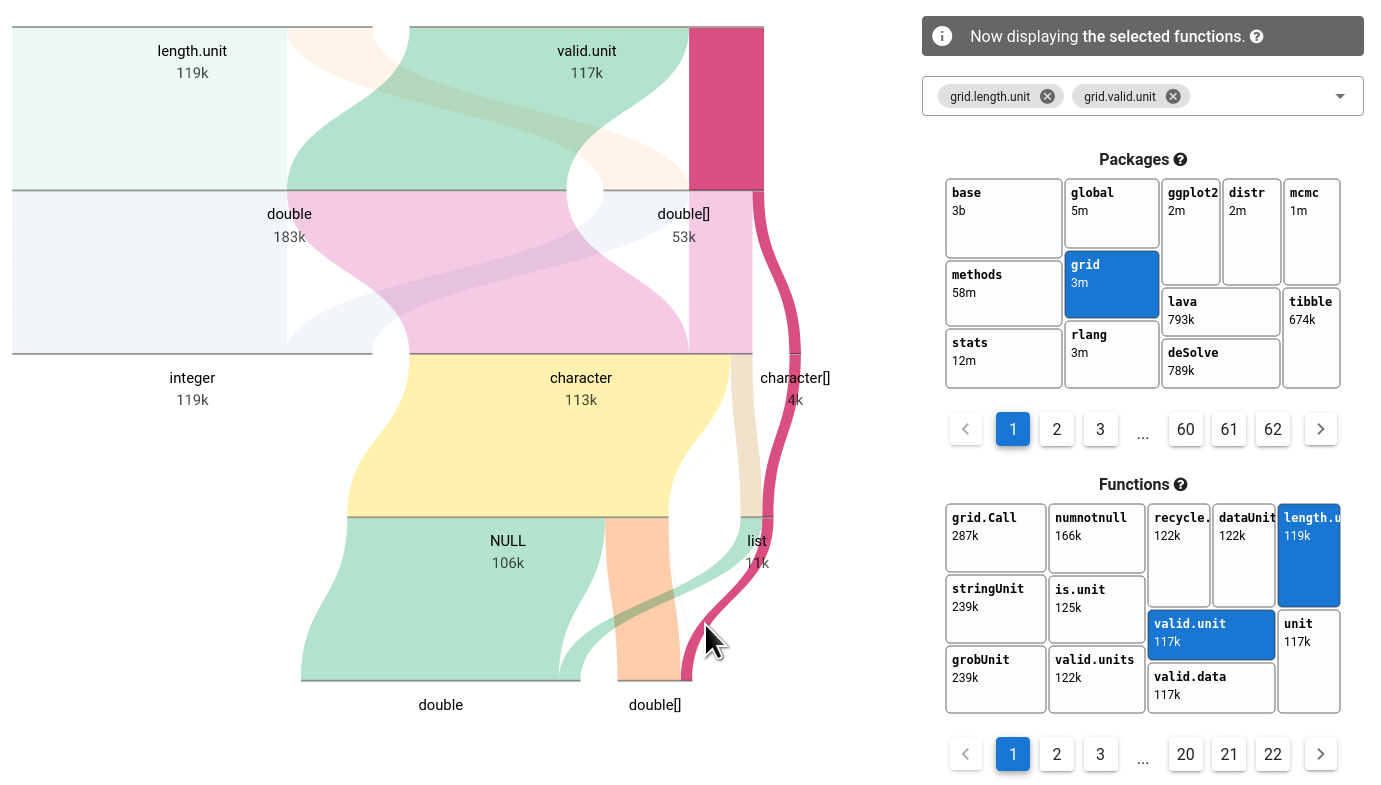
\includegraphics[width=\linewidth]{img/typevis.png}
 \caption{The main view of {\sc TypeVis}, with type flows on the left and the package hierarchy on the right.}
 \label{fig:typevis}
\end{figure*}

\begin{figure}[tb]
 \centering
 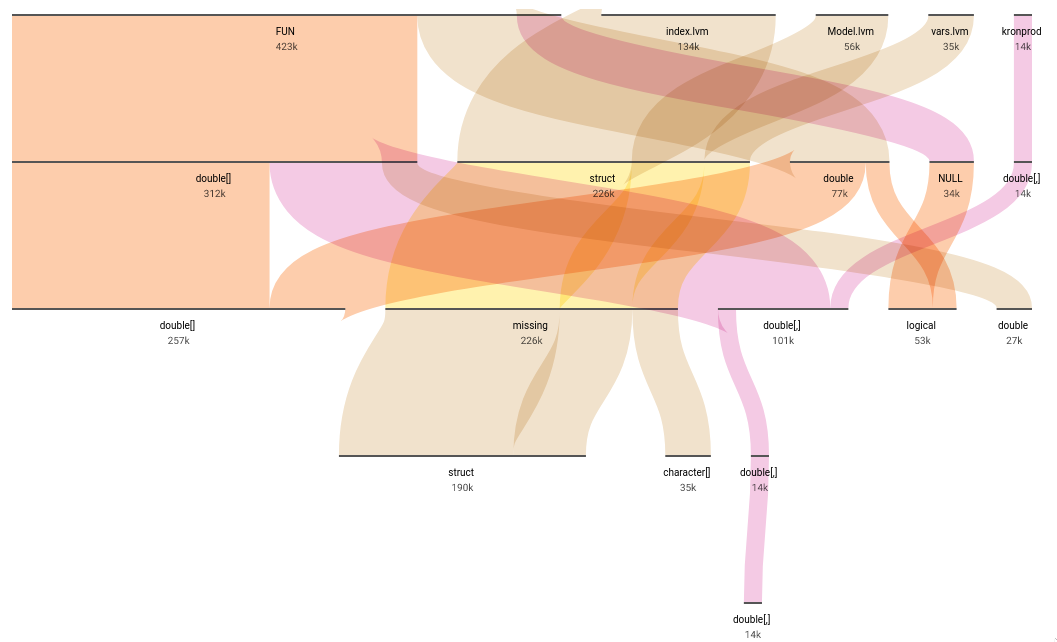
\includegraphics[width=\columnwidth]{img/no_decross.png}
 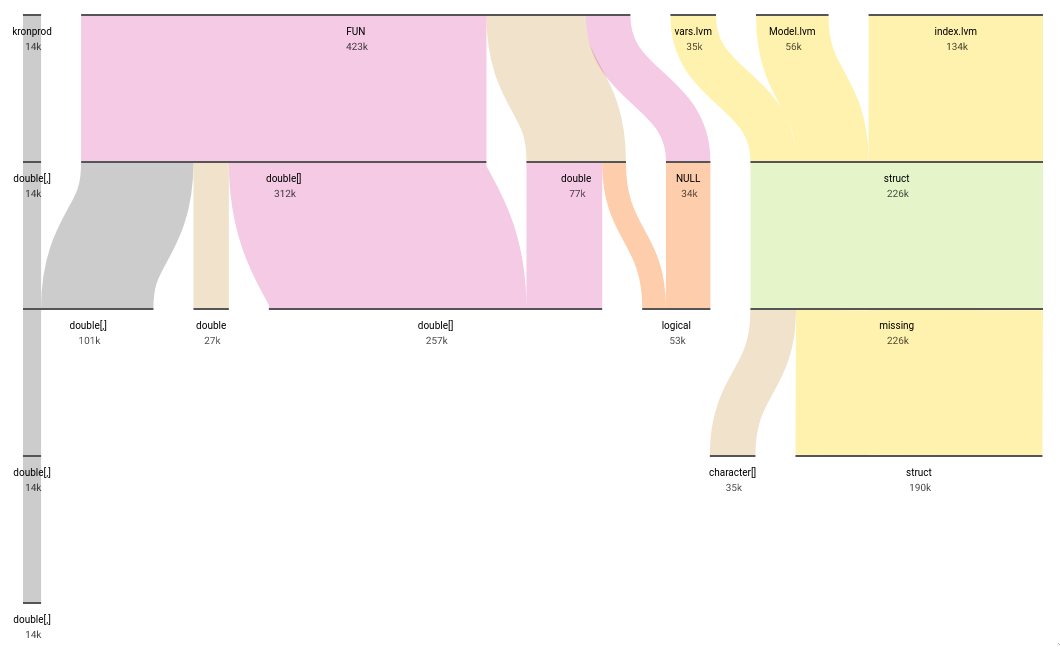
\includegraphics[width=\columnwidth]{img/decross.png}
 \caption{Comparison of type flows without decrossing (above) and with decrossing (below).}
 \label{fig:decross}
\end{figure}

%%

\section{Discussion}

\todo{Should say this is not R specific. Point limitations.}

%%

\section{Conclusion and Future Work}

\todo{Write.}

%%
%\section{Using the Style Template}
%
%\begin{itemize}
%\item If you receive compilation errors along the lines of ``\texttt{Package ifpdf Error: Name clash, \textbackslash ifpdf is already defined}'' then please add a new line ``\texttt{\textbackslash let\textbackslash ifpdf\textbackslash relax}'' right after the ``\texttt{\textbackslash documentclass[journal]\{vgtc\}}'' call. Note that your error is due to packages you use that define ``\texttt{\textbackslash ifpdf}'' which is obsolete (the result is that \texttt{\textbackslash ifpdf} is defined twice); these packages should be changed to use ifpdf package instead.
%\item The style uses the hyperref package, thus turns references into internal links. We thus recommend to make use of the ``\texttt{\textbackslash autoref\{reference\}}'' call (instead of ``\texttt{Figure\~{}\textbackslash ref\{reference\}}'' or similar) since ``\texttt{\textbackslash autoref\{reference\}}'' turns the entire reference into an internal link, not just the number. Examples: \autoref{fig:sample} and \autoref{tab:vis_papers}.
%\item The style automatically looks for image files with the correct extension (eps for regular \LaTeX; pdf, png, and jpg for pdf\LaTeX), in a set of given subfolders (figures/, pictures/, images/). It is thus sufficient to use ``\texttt{\textbackslash includegraphics\{CypressView\}}'' (instead of ``\texttt{\textbackslash includegraphics\{pictures/CypressView.jpg\}}'').
%\item For adding hyperlinks and DOIs to the list of references, you can use ``\texttt{\textbackslash bibliographystyle\{abbrv-doi-hyperref-narrow\}}'' (instead of ``\texttt{\textbackslash bibliographystyle\{abbrv\}}''). It uses the doi and url fields in a bib\TeX\ entry and turns the entire reference into a link, giving priority to the doi. The doi can be entered with or without the ``\texttt{http://dx.doi.org/}'' url part. See the examples in the bib\TeX\ file and the bibliography at the end of this template.\\[1em]
%\textbf{Note 1:} occasionally (for some \LaTeX\ distributions) this hyper-linked bib\TeX\ style may lead to \textbf{compilation errors} (``\texttt{pdfendlink ended up in different nesting level ...}'') if a reference entry is broken across two pages (due to a bug in hyperref). In this case make sure you have the latest version of the hyperref package (i.\,e., update your \LaTeX\ installation/packages) or, alternatively, revert back to ``\texttt{\textbackslash bibliographystyle\{abbrv-doi-narrow\}}'' (at the expense of removing hyperlinks from the bibliography) and try ``\texttt{\textbackslash bibliographystyle\{abbrv-doi-hyperref-narrow\}}'' again after some more editing.\\[1em]
%\textbf{Note 2:} the ``\texttt{-narrow}'' versions of the bibliography style use the font ``PTSansNarrow-TLF'' for typesetting the DOIs in a compact way. This font needs to be available on your \LaTeX\ system. It is part of the \href{https://www.ctan.org/pkg/paratype}{``paratype'' package}, and many distributions (such as MikTeX) have it automatically installed. If you do not have this package yet and want to use a ``\texttt{-narrow}'' bibliography style then use your \LaTeX\ system's package installer to add it. If this is not possible you can also revert to the respective bibliography styles without the ``\texttt{-narrow}'' in the file name.\\[1em]
%DVI-based processes to compile the template apparently cannot handle the different font so, by default, the template file uses the \texttt{abbrv-doi} bibliography style but the compiled PDF shows you the effect of the \texttt{abbrv-doi-hyperref-narrow} style.
%\end{itemize}
%
%\section{Bibliography Instructions}
%
%\begin{itemize}
%\item Sort all bibliographic entries alphabetically but the last name of the first author. This \LaTeX/bib\TeX\ template takes care of this sorting automatically.
%\item Merge multiple references into one; e.\,g., use \cite{Max:1995:OMF,Kitware:2003} (not \cite{Kitware:2003}\cite{Max:1995:OMF}). Within each set of multiple references, the references should be sorted in ascending order. This \LaTeX/bib\TeX\ template takes care of both the merging and the sorting automatically.
%\item Verify all data obtained from digital libraries, even ACM's DL and IEEE Xplore  etc.\ are sometimes wrong or incomplete.
%\item Do not trust bibliographic data from other services such as Mendeley.com, Google Scholar, or similar; these are even more likely to be incorrect or incomplete.
%\item Articles in journal---items to include:
%  \begin{itemize}
%  \item author names
%	\item title
%	\item journal name
%	\item year
%	\item volume
%	\item number
%	\item month of publication as variable name (i.\,e., \{jan\} for January, etc.; month ranges using \{jan \#\{/\}\# feb\} or \{jan \#\{-{}-\}\# feb\})
%  \end{itemize}
%\item use journal names in proper style: correct: ``IEEE Transactions on Visualization and Computer Graphics'', incorrect: ``Visualization and Computer Graphics, IEEE Transactions on''
%\item Papers in proceedings---items to include:
%  \begin{itemize}
%  \item author names
%	\item title
%	\item abbreviated proceedings name: e.\,g., ``Proc.\textbackslash{} CONF\_ACRONYNM'' without the year; example: ``Proc.\textbackslash{} CHI'', ``Proc.\textbackslash{} 3DUI'', ``Proc.\textbackslash{} Eurographics'', ``Proc.\textbackslash{} EuroVis''
%	\item year
%	\item publisher
%	\item town with country of publisher (the town can be abbreviated for well-known towns such as New York or Berlin)
%  \end{itemize}
%\item article/paper title convention: refrain from using curly brackets, except for acronyms/proper names/words following dashes/question marks etc.; example:
%\begin{itemize}
%	\item paper ``Marching Cubes: A High Resolution 3D Surface Construction Algorithm''
%	\item should be entered as ``\{M\}arching \{C\}ubes: A High Resolution \{3D\} Surface Construction Algorithm'' or  ``\{M\}arching \{C\}ubes: A high resolution \{3D\} surface construction algorithm''
%	\item will be typeset as ``Marching Cubes: A high resolution 3D surface construction algorithm''
%\end{itemize}
%\item for all entries
%\begin{itemize}
%	\item DOI can be entered in the DOI field as plain DOI number or as DOI url; alternative: a url in the URL field
%	\item provide full page ranges AA-{}-BB
%\end{itemize}
%\item when citing references, do not use the reference as a sentence object; e.\,g., wrong: ``In \cite{Lorensen:1987:MCA} the authors describe \dots'', correct: ``Lorensen and Cline \cite{Lorensen:1987:MCA} describe \dots''
%\end{itemize}
%
%\section{Example Section}
%
%Lorem\marginpar{\small You can use the margins for comments while editing the submission, but please remove the marginpar comments for submission.} ipsum dolor sit amet, consetetur sadipscing elitr, sed diam
%nonumy eirmod tempor invidunt ut labore et dolore magna aliquyam erat,
%sed diam voluptua. At vero eos et accusam et justo duo dolores et ea
%rebum. Stet clita kasd gubergren, no sea takimata sanctus est Lorem
%ipsum dolor sit amet. Lorem ipsum dolor sit amet, consetetur
%sadipscing elitr, sed diam nonumy eirmod tempor invidunt ut labore et
%dolore magna aliquyam erat, sed diam
%voluptua~\cite{Kitware:2003,Max:1995:OMF}. At vero eos et accusam et
%justo duo dolores et ea rebum. Stet clita kasd gubergren, no sea
%takimata sanctus est Lorem ipsum dolor sit amet. Lorem ipsum dolor sit
%amet, consetetur sadipscing elitr, sed diam nonumy eirmod tempor
%invidunt ut labore et dolore magna aliquyam erat, sed diam
%voluptua. At vero eos et accusam et justo duo dolores et ea
%rebum. Stet clita kasd gubergren, no sea takimata sanctus est.
%
%\section{Exposition}
%
%Duis autem vel eum iriure dolor in hendrerit in vulputate velit esse
%molestie consequat, vel illum dolore eu feugiat nulla facilisis at
%vero eros et accumsan et iusto odio dignissim qui blandit praesent
%luptatum zzril delenit augue duis dolore te feugait nulla
%facilisi. Lorem ipsum dolor sit amet, consectetuer adipiscing elit,
%sed diam nonummy nibh euismod tincidunt ut laoreet dolore magna
%aliquam erat volutpat~\cite{Kindlmann:1999:SAG}.
%
%\begin{equation}
%\sum_{j=1}^{z} j = \frac{z(z+1)}{2}
%\end{equation}
%
%Lorem ipsum dolor sit amet, consetetur sadipscing elitr, sed diam
%nonumy eirmod tempor invidunt ut labore et dolore magna aliquyam erat,
%sed diam voluptua. At vero eos et accusam et justo duo dolores et ea
%rebum. Stet clita kasd gubergren, no sea takimata sanctus est Lorem
%ipsum dolor sit amet. Lorem ipsum dolor sit amet, consetetur
%sadipscing elitr, sed diam nonumy eirmod tempor invidunt ut labore et
%dolore magna aliquyam erat, sed diam voluptua. At vero eos et accusam
%et justo duo dolores et ea rebum. Stet clita kasd gubergren, no sea
%takimata sanctus est Lorem ipsum dolor sit amet.
%
%\subsection{Lorem ipsum}
%
%Lorem ipsum dolor sit amet (see \autoref{tab:vis_papers}), consetetur sadipscing elitr, sed diam
%nonumy eirmod tempor invidunt ut labore et dolore magna aliquyam erat,
%sed diam voluptua. At vero eos et accusam et justo duo dolores et ea
%rebum. Stet clita kasd gubergren, no sea takimata sanctus est Lorem
%ipsum dolor sit amet. Lorem ipsum dolor sit amet, consetetur
%sadipscing elitr, sed diam nonumy eirmod tempor invidunt ut labore et
%dolore magna aliquyam erat, sed diam voluptua. At vero eos et accusam
%et justo duo dolores et ea rebum. Stet clita kasd gubergren, no sea
%takimata sanctus est Lorem ipsum dolor sit amet. Lorem ipsum dolor sit
%amet, consetetur sadipscing elitr, sed diam nonumy eirmod tempor
%invidunt ut labore et dolore magna aliquyam erat, sed diam
%voluptua. At vero eos et accusam et justo duo dolores et ea
%rebum.
%
%\subsection{Mezcal Head}
%
%Lorem ipsum dolor sit amet (see \autoref{fig:sample}), consetetur sadipscing elitr, sed diam
%nonumy eirmod tempor invidunt ut labore et dolore magna aliquyam erat,
%sed diam voluptua. At vero eos et accusam et justo duo dolores et ea
%rebum. Stet clita kasd gubergren, no sea takimata sanctus est Lorem
%ipsum dolor sit amet. Lorem ipsum dolor sit amet, consetetur
%sadipscing elitr, sed diam nonumy eirmod tempor invidunt ut labore et
%dolore magna aliquyam erat, sed diam voluptua. At vero eos et accusam
%et justo duo dolores et ea rebum. Stet clita kasd gubergren, no sea
%takimata sanctus est Lorem ipsum dolor sit amet.
%
%\subsubsection{Duis Autem}
%
%Lorem ipsum dolor sit amet, consetetur sadipscing elitr, sed diam
%nonumy eirmod tempor invidunt ut labore et dolore magna aliquyam erat,
%sed diam voluptua. At vero eos et accusam et justo duo dolores et ea
%rebum. Stet clita kasd gubergren, no sea takimata sanctus est Lorem
%ipsum dolor sit amet. Lorem ipsum dolor sit amet, consetetur
%sadipscing elitr, sed diam nonumy eirmod tempor invidunt ut labore et
%dolore magna aliquyam erat, sed diam voluptua. At vero eos et accusam
%et justo duo dolores et ea rebum. Stet clita kasd gubergren, no sea
%takimata sanctus est Lorem ipsum dolor sit amet. Lorem ipsum dolor sit
%amet, consetetur sadipscing elitr, sed diam nonumy eirmod tempor
%invidunt ut labore et dolore magna aliquyam erat, sed diam
%voluptua. At vero eos et accusam et justo duo dolores et ea
%rebum. Stet clita kasd gubergren, no sea takimata sanctus est. Lorem
%ipsum dolor sit amet.
%
%\begin{figure}[tb]
% \centering % avoid the use of \begin{center}...\end{center} and use \centering instead (more compact)
% \includegraphics[width=\columnwidth]{paper-count-w-2015-new}
% \caption{A visualization of the 1990--2015 data from \autoref{tab:vis_papers}. The image is from \cite{Isenberg:2017:VMC} and is in the public domain.}
% \label{fig:sample}
%\end{figure}
%
%\subsubsection{Ejector Seat Reservation}
%
%Duis autem~\cite{Lorensen:1987:MCA}\footnote{The algorithm behind
%Marching Cubes \cite{Lorensen:1987:MCA} had already been
%described by Wyvill et al. \cite{Wyvill:1986:DSS} a year
%earlier.} vel eum iriure dolor in hendrerit
%in vulputate velit esse molestie consequat,\footnote{Footnotes
%appear at the bottom of the column.} vel illum dolore eu
%feugiat nulla facilisis at vero eros et accumsan et iusto odio
%dignissim qui blandit praesent luptatum zzril delenit augue duis
%dolore te feugait nulla facilisi. Lorem ipsum dolor sit amet,
%consectetuer adipiscing elit, sed diam nonummy nibh euismod tincidunt
%ut laoreet dolore magna aliquam erat volutpat.
%
%
%\paragraph{Confirmed Ejector Seat Reservation}
%
%Ut wisi enim ad minim veniam, quis nostrud exerci tation ullamcorper
%suscipit lobortis nisl ut aliquip ex ea commodo
%consequat~\cite{Nielson:1991:TAD}. Duis autem vel eum iriure dolor in
%hendrerit in vulputate velit esse molestie consequat, vel illum dolore
%eu feugiat nulla facilisis at vero eros et accumsan et iusto odio
%dignissim qui blandit praesent luptatum zzril delenit augue duis
%dolore te feugait nulla facilisi.
%
%\paragraph{Rejected Ejector Seat Reservation}
%
%Ut wisi enim ad minim veniam, quis nostrud exerci tation ullamcorper
%suscipit lobortis nisl ut aliquip ex ea commodo consequat. Duis autem
%vel eum iriure dolor in hendrerit in vulputate velit esse molestie
%
%
%\section{Conclusion}
%
%Lorem ipsum dolor sit amet, consetetur sadipscing elitr, sed diam
%nonumy eirmod tempor invidunt ut labore et dolore magna aliquyam erat,
%sed diam voluptua. At vero eos et accusam et justo duo dolores et ea
%rebum. Stet clita kasd gubergren, no sea takimata sanctus est Lorem
%ipsum dolor sit amet. Lorem ipsum dolor sit amet, consetetur
%sadipscing elitr, sed diam nonumy eirmod tempor invidunt ut labore et
%dolore magna aliquyam erat, sed diam voluptua. At vero eos et accusam
%et justo duo dolores et ea rebum. Stet clita kasd gubergren, no sea
%takimata sanctus est Lorem ipsum dolor sit amet. Lorem ipsum dolor sit
%amet, consetetur sadipscing elitr, sed diam nonumy eirmod tempor
%invidunt ut labore et dolore magna aliquyam erat, sed diam
%voluptua. At vero eos et accusam et justo duo dolores et ea
%rebum.

%% if specified like this the section will be committed in review mode
\acknowledgments{
The authors wish to thank A, B, and C. This work was supported in part by
a grant from XYZ.}

%\bibliographystyle{abbrv}
\bibliographystyle{abbrv-doi}
%\bibliographystyle{abbrv-doi-narrow}
%\bibliographystyle{abbrv-doi-hyperref}
%\bibliographystyle{abbrv-doi-hyperref-narrow}

\bibliography{main}
\end{document}
